%%%%%%%%%%%%%%%%%%%%%%%%%%%%%%%%%%%%%%%%%%%%%%%%%%%%%%%
%
% AUTHOR:lee-shun
%
% DESCRIBTION:第三章--自动驾驶仪控制逻辑
%
%
%%%%%%%%%%%%%%%%%%%%%%%%%%%%%%%%%%%%%%%%%%%%%%%%%%%%%%%

\chapter{自动驾驶仪控制逻辑}
\label{chap:single_control_logic}
正如前文所提到的:由于文中编队控制器基于领从方法(leader-follower method),因而领机的飞行完全是由预先给定的一系列航迹点以及自动驾驶仪
所决定的。并且,本文设计的的编队控制器是以现有开源自动驾驶仪PX4的内环为基础;因此,本章将首先介绍控制领机飞行的自动驾驶导航以
及位置模块的实现逻辑,之后将介绍固定翼无人机编队飞行至关重要的基础环节-----自动驾驶仪内环,即姿态内环的实现逻辑。
内环姿态驾驶仪使用的是开源自动驾驶仪PX4。PX4是一个为无人机或者其他无人系统设计的高度模块化、可定制化的开源自动驾驶仪软件系统;
PX4软件本身提供了丰富的应用程序接口(API)以及软件开发工具包(SDK),可以与$ROS$等机器人操作系统进行数据交互。下图展示了$PX4$
的软件架构以及各个模块之间的交互关系:
\begin{figure}[H]
    \centering
    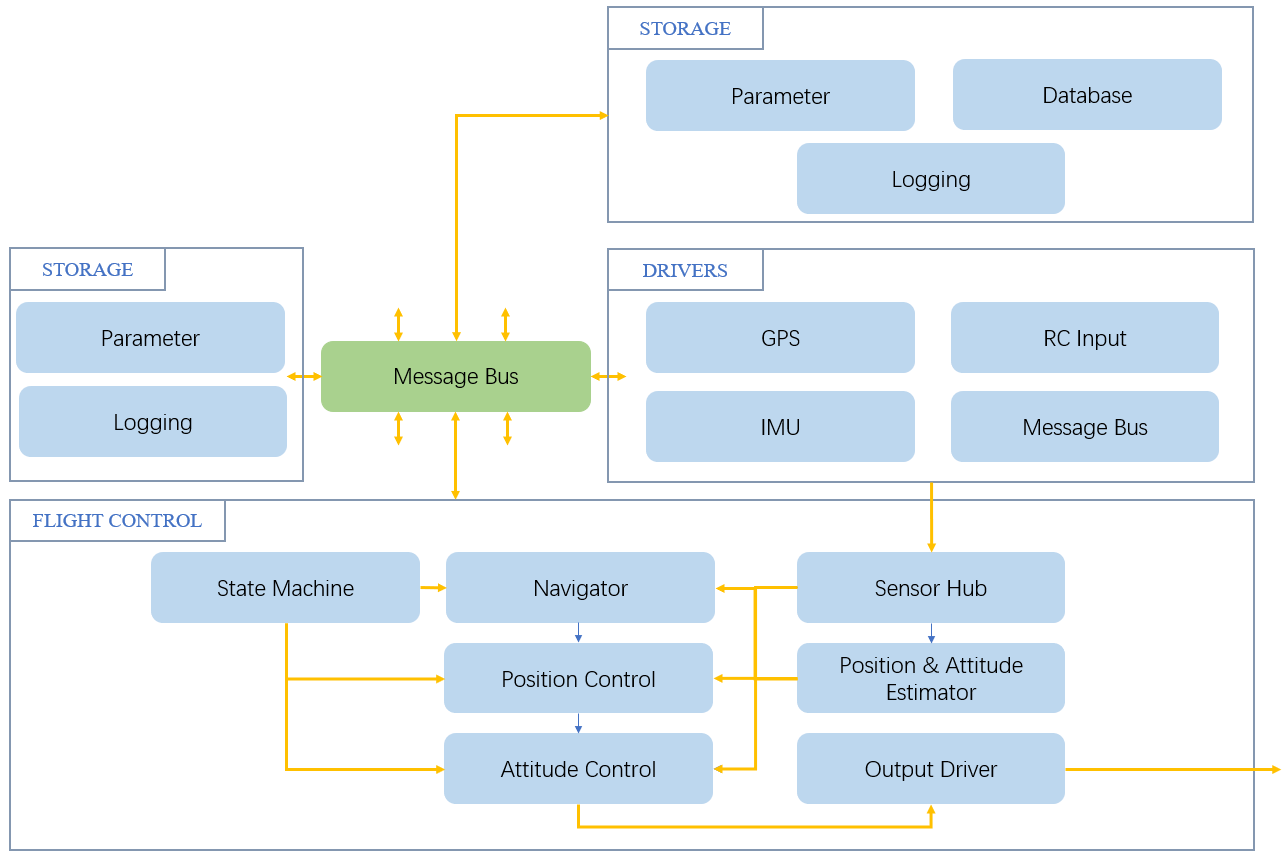
\includegraphics[width=0.8\textwidth]{figures/c4/PX4_archticher.png}
    \caption{PX4软件架构}\label{fig:PX4_archticher.png}
\end{figure}
\section{导航以及位置外环实现逻辑}
所谓导航模块(Naigator),其功能是产生相应的期望位置航点。编队中领机按照给定的航迹飞行,导航模块则根据给定的航点以及无人机的位置不断得出当前位置
下的期望航点。位置外环的主要功能是接受来自导航模块的期望位置,再结合无人机的当前位置,按照给定的导航算法,产生姿态内环的所接受的
期望姿态以及期望推力值。位置外环将无人机的运动分为竖直与水平平面的运动,并在上述两个平面内分别设计位置控制器;竖直平面控制器选用
TECS控制器,水平平面选用L1控制器。下面将简要介绍上述两种控制器的控制逻辑:
\subsection{TECS控制器控制逻辑}
所谓总能量控制(total energy control)是将无人机的速度以及高度计算得到相应的动能以及势能作为直接控制对象,应用PID控制器对动能与势能的和(total energy)
以及动能与势能的转化(total energy balance)进行控制,计算得到无人机期望俯仰角以及期望推力的控制器。飞机作为一个动力学系统,其机械能来自推力做功的输入,因而总能量控制对应着期望推力;与之对应的俯仰角控制是能量守恒的,
可作为动能向势能(反之亦然)的转化途径,对此种能量转化的控制对应着期望俯仰角。下面简要介绍TECS控制器的计算过程:
\\
无人机的总能量为:
\begin{equation}
    E_T=\frac{1}{2}mV_T^2+mgh
    \label{ET}
\end{equation}
对上式两边微分,可得到总能量变化率:
\begin{equation}
    \dot{E_T}=mV_T\dot{V_T}+mg\dot{h}
    \label{ET_rate}
\end{equation}
由此可得单位总能量变化率:
\begin{equation}
    \dot{E}=\frac{\dot{E}_{T}}{m g V_{T}}=\frac{\dot{V}_{T}}{g}+\frac{\dot{h}}{V_{T}}=\frac{\dot{V}_{T}}{g}+\sin \gamma
    \label{specif_ET_rate}
\end{equation}
更换式\ref{point_dynamaic}第一式形式,可得到:
\begin{equation}
    T-D=m g\left(\frac{\dot{V}_{T}}{g}+\sin \gamma\right)
    \label{point_dynamaic_change}
\end{equation}
由此可得:
\begin{equation}
    \Delta T=m g\left(\frac{\dot{V}_{T}}{g}+sin\gamma\right)
    \label{thrust}
\end{equation}
关于能量转化,定义:
\begin{equation}
    B=m g h-\frac{1}{2} m V_{T}^{2}
\end{equation}
能量转化率为:
\begin{equation}
\dot{B}=sin\gamma-\frac{\dot{V}_{T}}{g}
\end{equation}
这里参照开源自驾仪PX4内部的TECS控制器设计方法,总能量环和能量分配环的控制逻辑框图如下所示:
\begin{figure}[H]
    \centering
    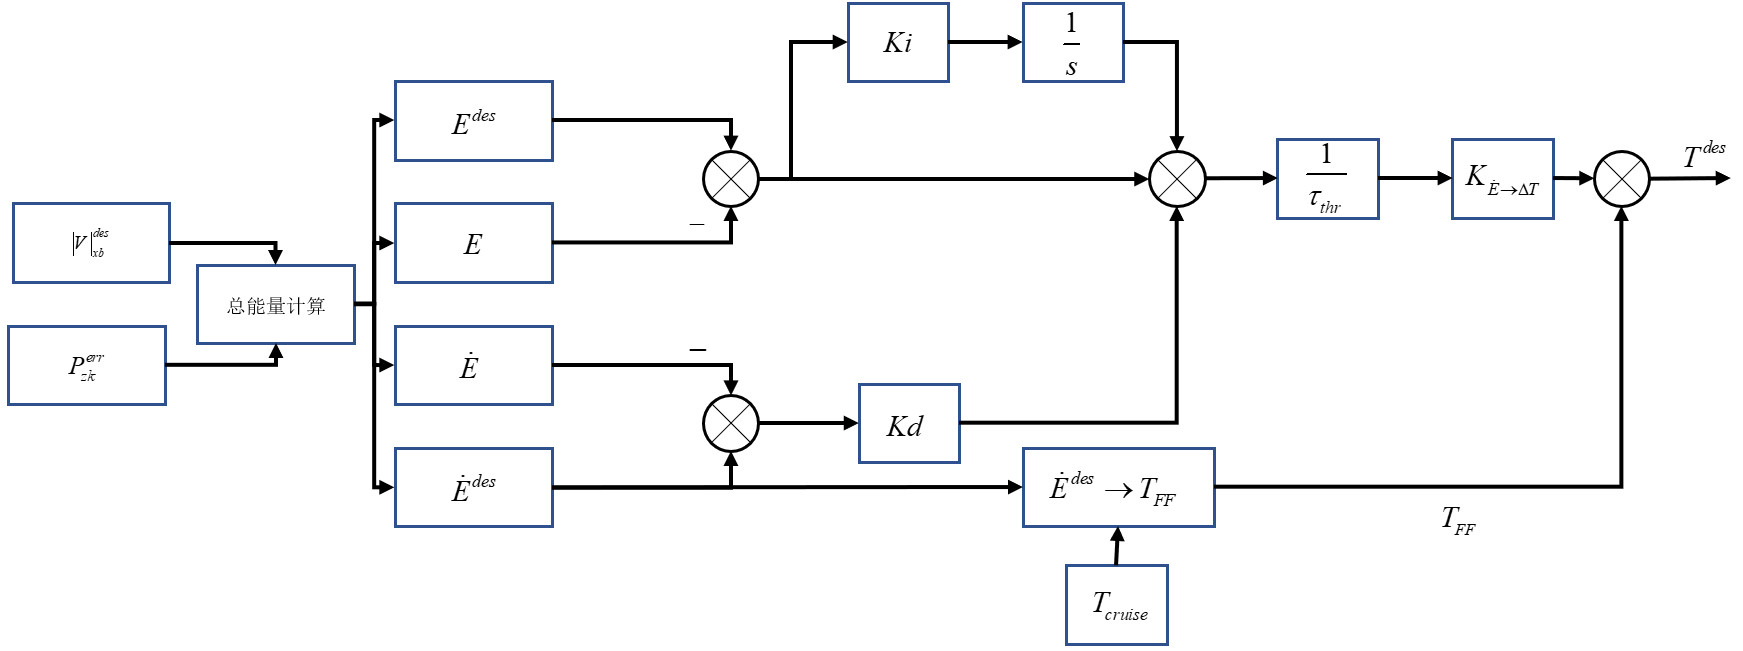
\includegraphics[width=0.9\textwidth]{figures/c3/TECS_throttle.jpg}
    \caption{总能量环}\label{fig:total_energy}
\end{figure}
\begin{figure}[H]
    \centering
    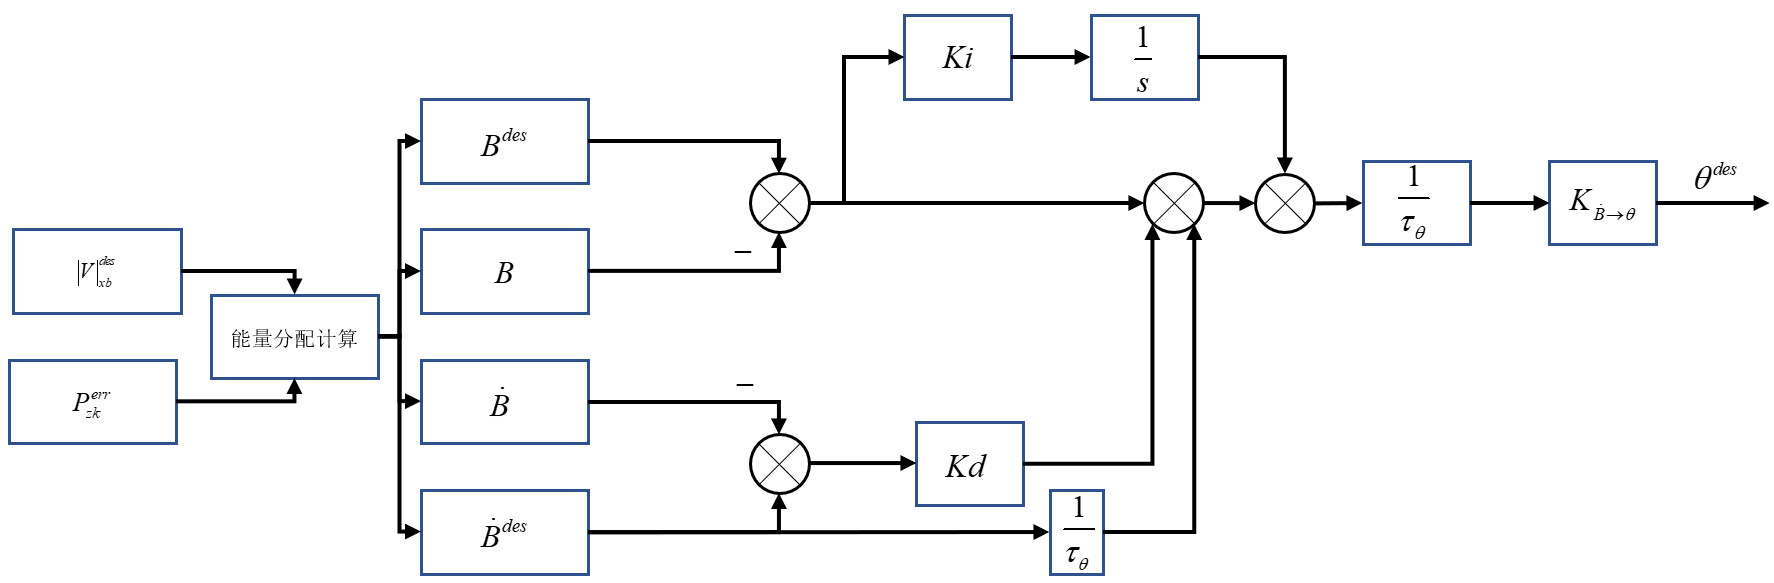
\includegraphics[width=0.9\textwidth]{figures/c3/TECS_pitch.jpg}
    \caption{能量分配环}\label{fig:balance_energy}
\end{figure}
图\ref{fig:total_energy}中,$K_i,K_d,T_{FF},\tau_{thr},K_{\dot{E}\rightarrow\Delta T}$分别为积分项,微分项比例系数,
油门前馈项,油门时间常数以及比例向项系数。
图\ref{fig:balance_energy}中,$K_i,K_d,\tau_{\theta},K_{\dot{B}\rightarrow\Delta \theta}$分别为积分项,微分项比例系数,俯仰角时间常数以及比例向项系数。
\subsection{L1控制器实现逻辑}
所谓L1控制器是Sanghyuk Park等人在文献\cite{Park_2004}中提出的一种非线性航迹追踪方法的一种工程实现。Sanghyuk Park在此文中对于此种
控制器的稳定性做了详细的证明,并在不同飞行状态下对此种控制器与传统线性的控制器控制效果做出了完整对比。下面仅作简要介绍:
应用L1控制器分为两步:首先应选取在所控制无人机之前的期望航迹之上的并且距离无人机当前位置为L1距离的参考点,如下图\cite{Park_2004}所示:
\begin{figure}[H]
    \centering
    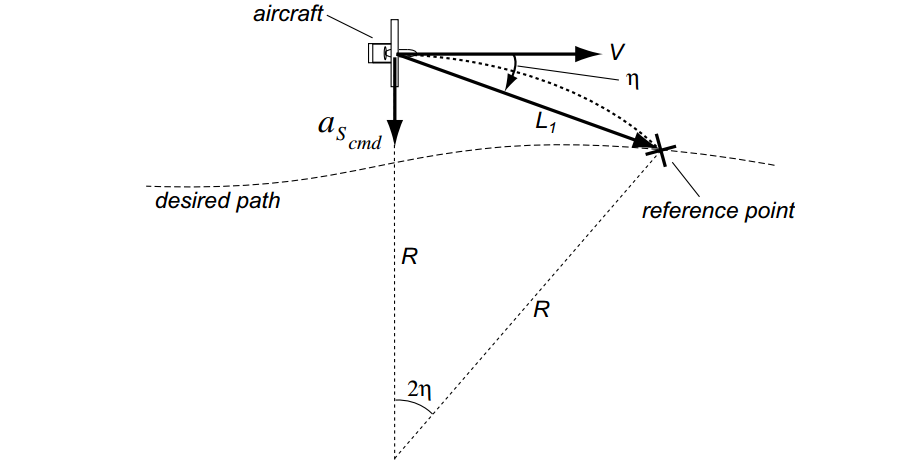
\includegraphics[width=0.75\textwidth]{figures/c3/L1_control}
    \caption{L1控制逻辑图}\label{fig:L1_control}
\end{figure}
之后期望向心加速度$a_{s_{cmd}}$由下式\cite{Park_2004}给出,此式即为L1控制器的导引律。
\begin{equation}
    a_{s_{cmd}}=2\frac{V^2}{L_1}sin\eta
\end{equation}
最终的控制效果为:
\begin{figure}[H]
    \centering
    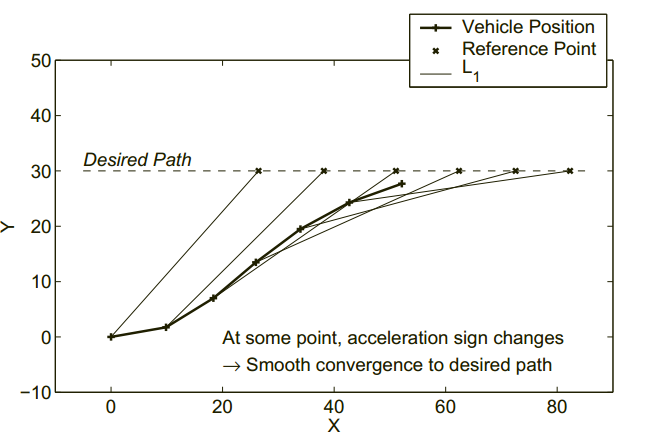
\includegraphics[width=0.75\textwidth]{figures/c3/L1_eff}
    \caption{L1控制器控制效果}\label{fig:c3-L1_eff}
\end{figure}
在做曲线航迹追踪时,按照Sanghyuk Park等人的分析,控制律将近似为PD控制器。
之后,按照实际应用的需要,并参考Paul Riseborough, Brandon Jones 和 Andrew Tridgell等人为另一款开源无人机自动驾驶仪APM的L1
控制器设计,将上述导引律做如下改动:
\begin{enumerate}
    \item 显式表示控制律中的频率以及阻尼。
    \item 显式表示跟踪角度。
    \item 可以使用小于L1长度的盘旋半径。
    \item 修改原始圆形追踪控制律,使用PD控制器使得盘旋时可使用小于L1长度的盘旋半径。
    \item 修改控制逻辑可以分别调整L1控制器的阻尼比以及周期。\label{enu:period}
\end{enumerate}
对于较为关键的第\ref{enu:period}项,最终的$L1$长度选择可由下式表示:
 \begin{equation}
     L_1 = \frac{V}{\pi T_{L1} \xi_{L1}}
\end{equation}
\section{姿态内环控制原理}
总体而言,内环的控制器为串级PID,分为角度环,角速度环以及角加速度环,其控制框图如下所示:
\begin{figure}[H]
    \centering
    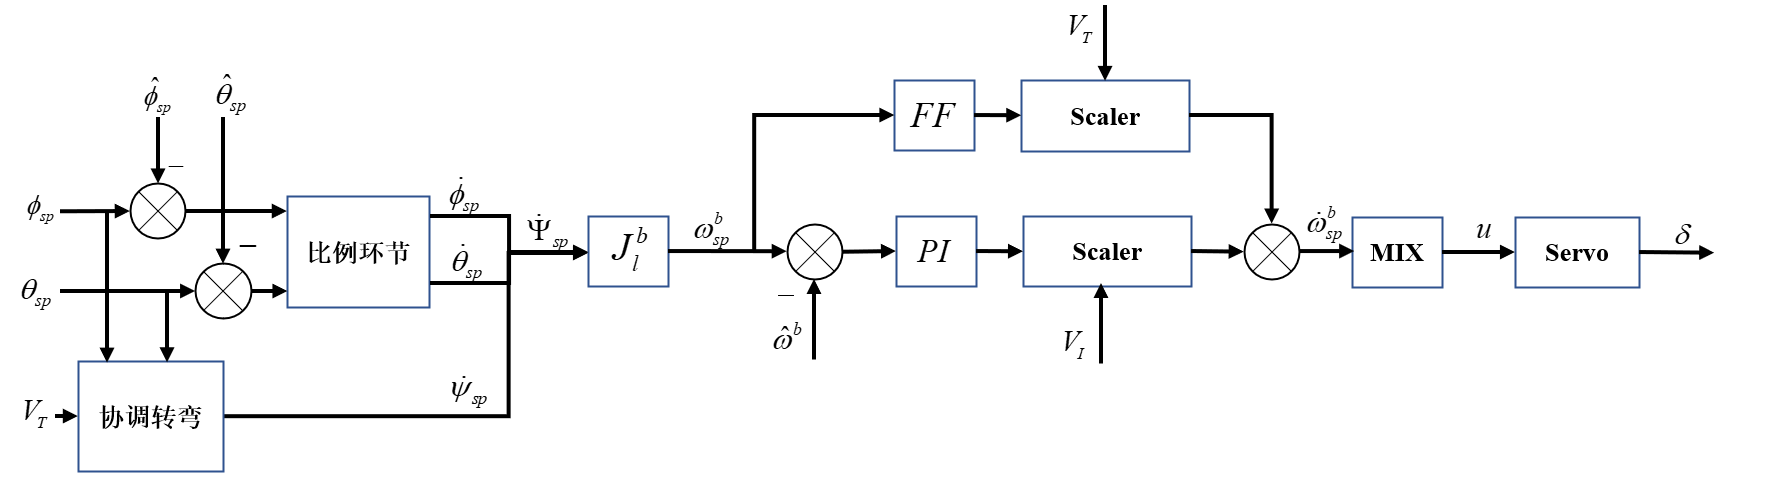
\includegraphics[width=0.90\textwidth]{figures/c3/attitude_inner_loop}
    \caption{姿态内环控制原理框图}\label{c3-attitude_inner_loop}
\end{figure}
其中,$\phi_{sp}$,$\theta_{sp}$,$\psi_{sp}$分别为滚转角、俯仰角以及偏航角期望值;$\dot{\phi}_{sp}$,$\dot{\theta}_{sp}$,$\dot{\psi}_{sp}$
分别为姿态角速度期望值;$\dot{\Psi}_{sp}$为上述期望姿态角速度所组成的三维向量;$J^{b}_l$为无人机由惯性系到机体系的转换矩阵;
$V_T$、$V_I$分别为无人机真实空速(true air speed)以及指示空速(indicator air speed);形如“$\hat{\theta}$”的符号为相应
物理量的估计值。

如上图所示,姿态驾驶仪的外环计算期望姿态与估计姿态之间的误差,经过比例控制之后产生角速度期望值。
内环计算速率误差并且利用比例积分控制产生期望的角加速度期望值。

之后,控制面的控制角位置的产生则由期望的角加速度以及无人机系统的先验知识,即控制分配关系所产生。
进一步的,因为在高速下的控制面效率要大于低速下,因而控制器中设计“巡航速度”这一参数来计算空速的影响。

控制器中的前馈增益用来补偿空气动力学阻尼。体轴系下的力矩基本上由控制面以及气动阻尼产生。因此,为了保持滚转角速率为常数,
空气阻尼力矩与控制力矩大小相等,方向相反,因此此种阻尼可由前馈项计算得出。

内环控制器中的滚转以及俯仰通道的控制有者相似的结构,但是在偏航通道上,偏航角度度的期望值是直接由飞机协调转弯条件得出,
以降低在飞机转弯时的衡侧向加速度,具体请参见文献\cite{Fangzhenping2005}
